\section{Architecture Integration}

\subsection{Model Support}

\begin{table}[H]
\centering
\small
\begin{tabular}{llllll}
\toprule
\textbf{Architecture} & \textbf{Attention} & \textbf{Nested?} & \textbf{RoPE?} & \textbf{GQA?} & \textbf{Verified} \\
\midrule
DistilBERT & Flat & No & No & No &  \\
RoBERTa & Nested & Yes & No & No &  \\
GPT-2 & Causal & No & No & No &  \\
Qwen3.5 & GQA+RoPE & No & Yes & Yes & partial \\
\bottomrule
\end{tabular}
\end{table}

\subsection{Weight Extraction}

\subsubsection{DistilBERT (Flat)}
\begin{lstlisting}
q\_w = src.q\_lin.weight
k\_w = src.k\_lin.weight
v\_w = src.v\_lin.weight
o\_w = src.out\_lin.weight
is\_nested\_encoder = False
\end{lstlisting}

\subsubsection{RoBERTa (Nested)}
\begin{lstlisting}
q\_w = src.self.query.weight
k\_w = src.self.key.weight
v\_w = src.self.value.weight
# output.dense applied by outer module
is\_nested\_encoder = True
\end{lstlisting}

\subsubsection{GPT-2 (Conv1D)}
\begin{lstlisting}
w = src.c\_attn.weight.T
q\_w, k\_w, v\_w = w.chunk(3, dim=0)
o\_w = src.c\_proj.weight.T
\end{lstlisting}

\subsubsection{Qwen (GQA + RoPE)}
Direct copy with GQA-aware dims.

\subsection{Injection}

\begin{lstlisting}
def inject\_cluster(layer, cfg, comp\_config, old\_attn):
    new = ClusterAttention(
        config=cfg,
        comp\_config=comp\_config,
        pretrained\_attn=old\_attn,
        num\_clusters=16,
        n\_iters=3,
        window\_size=32,
    )
    if hasattr(layer, "attention"):
        if hasattr(layer.attention, "self"):
            layer.attention.self = new
        else:
            layer.attention = new
    return new
\end{lstlisting}

\subsection{Causal Masking}

For decoders, ClusterFormer uses \textbf{exact causal attention}, not clustering:

\begin{lstlisting}
if is\_decoder:
    scores = Q @ K.T / sqrt(d\_h)
    scores = scores.masked\_fill(~causal\_tril, -10000)
    attn = softmax(scores)
    out = attn @ V
\end{lstlisting}

\textbf{Rationale.} Clustering introduces a global mixing effect that can leak 
future information even with causal masking on keys. For stability we 
use standard exact attention for decoder paths.

\subsection{RoPE}

Partial RoPE (Qwen3.5 with rotary\_dim \textless{} head\_dim) is supported via slicing 
the first \texttt{rotary\_dim} coordinates.

\subsection{GQA}

\begin{lstlisting}
if self.kv\_repeat \textgreater{} 1:
    K = repeat\_kv(K, self.kv\_repeat)
    V = repeat\_kv(V, self.kv\_repeat)
\end{lstlisting}

\subsection{Registry}

\begin{lstlisting}
@ATTENTION\_REGISTRY.register("cluster")
@ATTENTION\_REGISTRY.register("cluster\_attention")
class ClusterAttention(BaseAttention):
    ...
\end{lstlisting}

\subsection{Failure Modes}

\begin{table}[H]
\centering
\small
\begin{tabular}{lll}
\toprule
\textbf{Failure} & \textbf{Detection} & \textbf{Response} \\
\midrule
Missing weights & \texttt{copy\_weights} raises & Return None \\
Empty clusters & \texttt{counts == 0} & Mask logit to -inf \\
NaN in cdist & \texttt{torch.nan\_to\_num} & Replace with 0 \\
Zero Frobenius & Check \textless{} 1e-4 & Raise error \\
\bottomrule
\end{tabular}
\end{table}

\subsection{Numerical Stability}

\begin{lstlisting}

---
\end{lstlisting}

\begin{figure}[H]
\centering
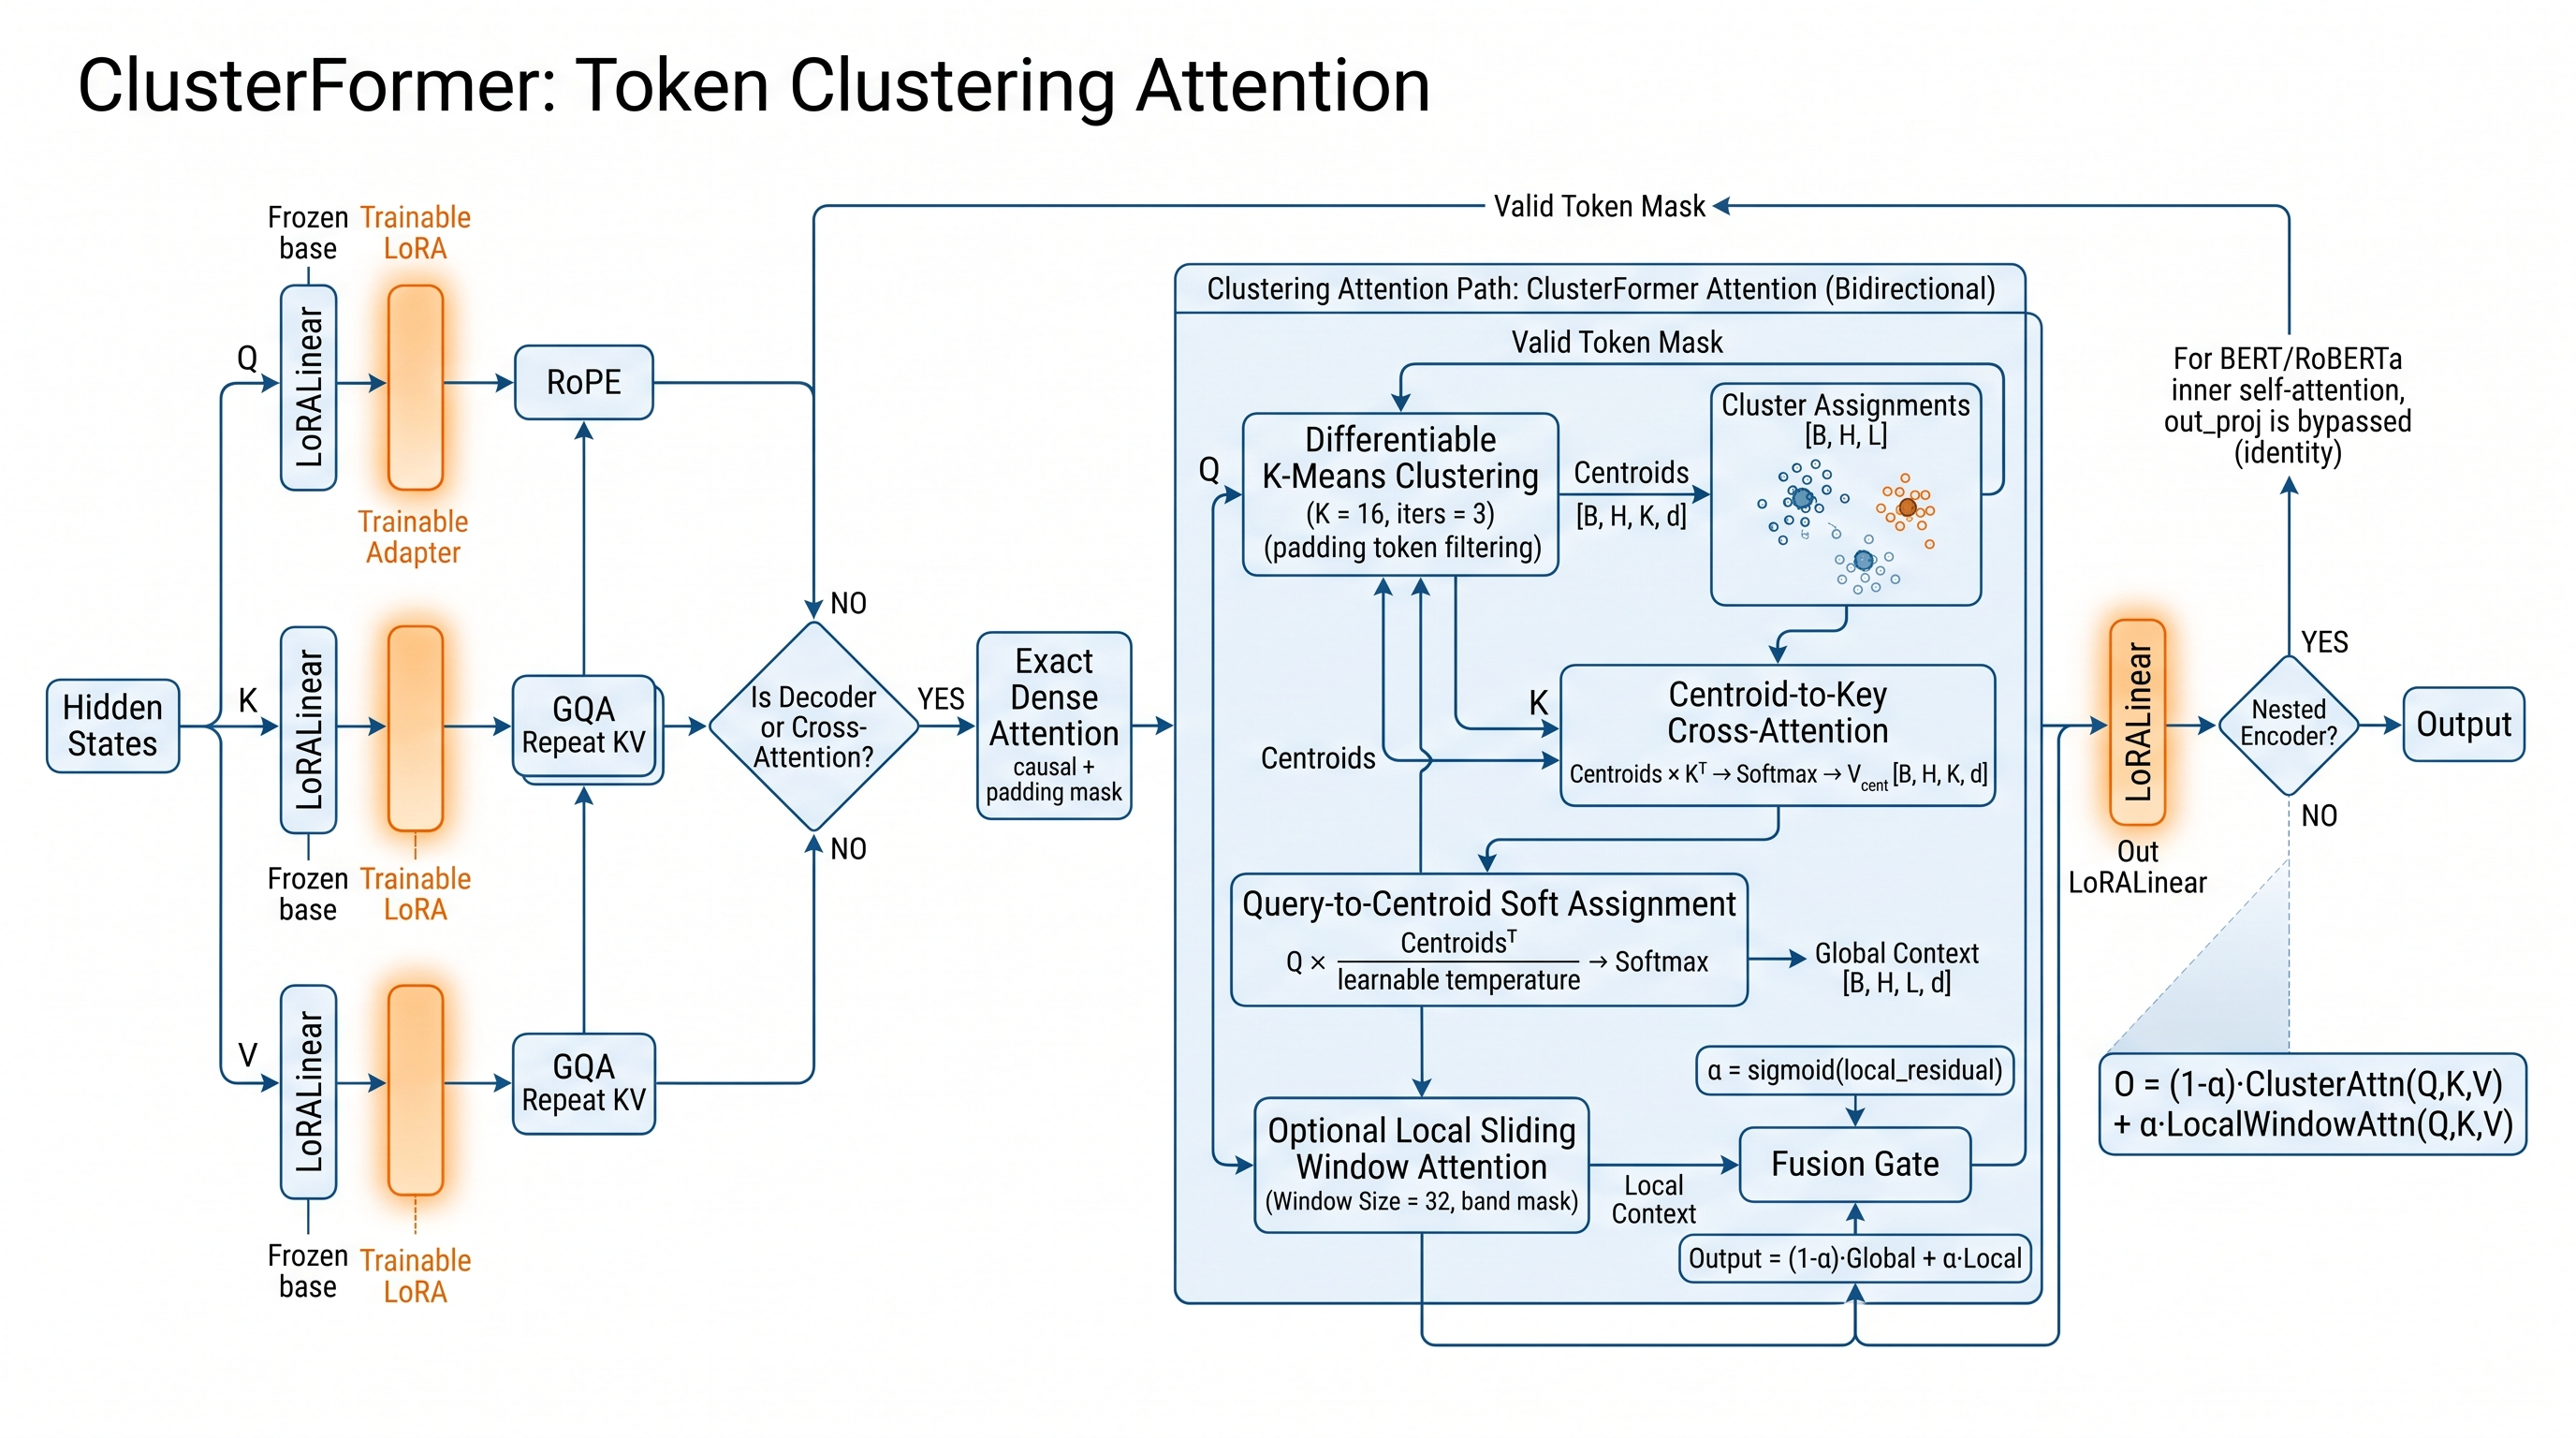
\includegraphics[width=\linewidth]{figures/architecture.jpeg}
\caption{High-level architectural diagram of cluster.}
\label{fig:arch_cluster}
\end{figure}

